\chapter{Marco Teórico}

Este capítulo va a poner en contexto al lector con respecto a conceptos básicos de criptografía, definir y explicar los algoritmos que van a ser implementados en el FPGA, y realizar una breve explicación sobre características de un FPGA para explicar el porqué de la escogencia de los parámetros que van a ser analizadas.

\section{Conceptos Básicos}
Según la \cite{raeCriptografia} la criptografía se define como
\begin{center}
    \begin{minipage}{0.9\linewidth}
        \vspace{5pt}%margen superior de minipage
        {\small
            \emph{Arte de escribir con clave secreta o de un modo enigmático.}
        }
 		\vspace{5pt}%margen inferior de la minipage
    \end{minipage}
\end{center}
El mensaje que se desea transmitir es llamado \textit{texto plano} o simplemente \textit{mensaje}. Este mensaje pasa por un proceso donde se disfraza el texto plano en un \textit{texto cifrado}, el proceso se denomina \textit{cifrado}\footnote{Según el ISO 7498-2 los términos correctos para encriptar y desencriptar son cifrar y descifrar respectivamente.}. El proceso inverso donde se toma un texto cifrado en un texto plano se denomina \textit{descifrado} \citep{bruce}. 

El texto plano o mensaje se denota por la letra M o P, el texto cifrado se denota por la letra C, la función o algoritmo que cifra se denota por E y la que descrifa se denota por D. Un algoritmo criptográfico corresponde a la función matemática para cifrar y descrifrar.
\newline
Se muestra en las Ecuaciones \eqref{eqCifrado} y \eqref{eqDescifrado} las relaciones entre estas notaciones. Note como al aplicarle la función de cifrado al texto plano se obtiene el texto cifrado y como al aplicarle la función de descifrado al texto cifrado se obtiene el texto plano. Finalmente se debe cumplir la identidad que describe la Ecuación \eqref{eqCifraDescifra} \citep{bruce}.
\begin{equation} \label{eqCifrado}
E(M) = C
\end{equation}
\begin{equation} \label{eqDescifrado}
D(C) = M
\end{equation}
\begin{equation} \label{eqCifraDescifra}
D(E(M)) = M
\end{equation}


La importancia de la criptografía transciende más allá de brindar la confidencialidad en la comunicación, la criptografía también cumple con la siguientes tareas:
\begin{itemize}
\item Autenticación: El receptor del mensaje debe de poder conocer y asegurar el emisor del mensaje, esto para que un tercero no pueda adjudicarse la identidad del emisor.
\item Integridad: El receptor tiene que poder asegurarse que el mensaje no fue cambiado en el transito del mismo. Esto para que un tercero no pueda cambiar el contenido enviado por el emisor sin que el receptor lo sepa.
\item \textit{Non-repudiation}: El emisor del mensaje no puede negar que el mensaje fue enviado por él. 
\end{itemize}

\section{Sistema criptográfico (\textit{criptosistema})}
Cuando la seguridad del algoritmo se basa en como procede el algoritmo, se denomina \textit{algoritmo restringido}. Este tipo de algoritmos son poco utilizados en la actualidad debido al gran problema que presentan. Tomemos de ejemplo que un grupo de usuarios decide utilizar un algoritmo criptográfico restringido para sus comunicaciones, se tendrá una comunicación segura hasta que alguno de los miembros decida salirse del grupo, ya que el usuario al no pertenecer más al grupo, no le importa mantener en secreto el algoritmo y puede distribuirlo para que terceros intercepten las comunicaciones. Así cada vez que un miembro deja el grupo, se debe proceder a cambiarse a todo un nuevo algoritmo lo cual puede tornarse una labor complicada. También ocurre el problema que si se logra obtener un algoritmo equivalente para cifrar los datos, se debe migrar a un nuevo algoritmo.

En cambio, la criptografía moderna \citep{denning} agrega el concepto de \textit{llave} donde se tiene un algoritmo el cual toma como parámetros de entrada una llave y el texto plano o cifrado, y cifra o descifra el mismo de forma correcta, únicamente si se tiene la llave correcta. El esquema descrito anteriormente se muestra en la Figura \ref{figExplicacionSistemaCripto}. Retomando el ejemplo anterior, el grupo solamente necesitaría cambiar de llave cuando un miembro se va, facilitando el uso del cifrado y manteniendo las comunicaciones secretas. 

Estos conceptos viene a definir lo que actualmente se conoce como sistema criptográfico o \textit{criptosistema}. Según \cite{denning}, un criptosistema cuenta con 5 componentes:
\begin{itemize}
\item Un espacio de textos planos o mensajes ($M$)
\item Un espacio de textos cifrados ($C$)
\item Un espacio de llaves ($k$)
\item Una familia de \textit{transformaciones de cifrado}: $E_K: M\rightarrow C$ donde $K \epsilon  k$
\item Una familia de \textit{transformaciones de descrifrado}: $C_K: C\rightarrow M$ donde $K \epsilon  k$
\end{itemize} 


Se entiende como \textit{espacio} el conjunto de posibles valores para la variable dada, sea esta M, C o K.
Y una familia de transformaciones corresponde a todos los posibles mapeos que se pueden realizar de un espacio a otro (de $M$ a $C$ o viceversa) con todos los valores contenidos en el espacio $k$.

\begin{figure}
	\centering
	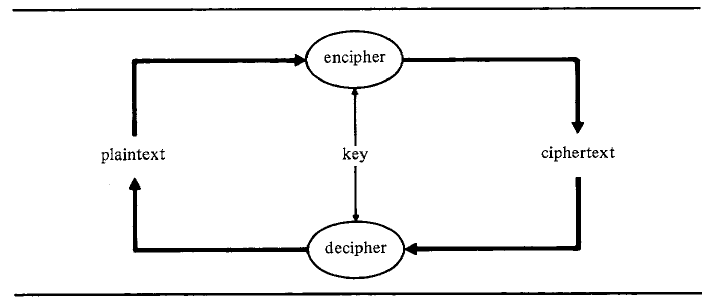
\includegraphics[width=0.8\textwidth]{./images/figExplicacionSistemaCripto}
	\caption{Descripción gráfica de un sistema criptográfico \citep{denning}.}
	\label{figExplicacionSistemaCripto}
\end{figure}


En la actualidad se trabaja la criptografía sobre computadoras, es decir, cifrando y descrifrando bits, los cuales pueden tener diferentes significados, ya sea una imagen, un texto, un programa, etc. Esto significa que en la actualidad no se trabaja sobre caracteres del alfabeto o símbolos, sino más bien sobre 1's y 0's. Esto toma relevancia ya que al tener solo dos símbolos para cifrar, los algoritmos se vuelven más complejos por la falta de alternativas para sustituir un símbolo por otro.

Antiguamente la criptografía se basaba en caracteres que eran sustituidos o traspuestos por otros caracteres. Esto corresponde a cifrados de sustitución y de transposición, los cuales continúan siendo la base de la criptografía pero basado en los dos símbolos del sistema binario.

Como se explicó anteriormente el cifrado de sustitución se basa en tomar un caracter del texto plano y sustituirlo por otro caracter. Para descrifrar el texto cifrado simplemente se sustituyen de vuelta los caracteres y listo.

Según \cite{bruce}, en la criptografía clásica existen 4 tipos de cifrado por sustitución:
\begin{itemize}
\item Cifrado de sustitución simple: Una sustitución de uno a uno entre cada caracter del texto plano y el texto cifrado.
Ejemplos de este tipo de sustitución son el famoso cifrado de César y el ROT13 utilizado en UNIX.

\item Cifrado de sustitución homofónico: Una sustición de uno a muchos. Un caracter del texto plano, por ejemplo A, puede ser sustituido por varios caracteres en el texto crifado, por ejemplo ``5'', ``13'', ``43''. Observe la Figura \ref{figExampleHomophonicCipher} donde se presenta una serie de posibles asignaciones de números a las letras del mensaje PLAIN PILOT y un posible texto cifrado haciendo uso de este tipo de cifrado.

\begin{figure}
	\centering
	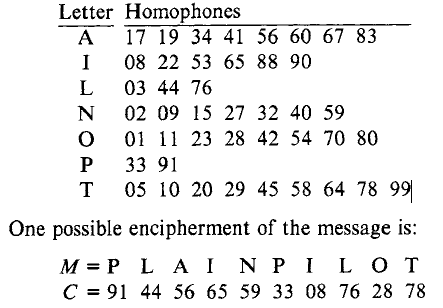
\includegraphics[width=0.6\textwidth]{./images/figExampleHomophonicCipher}
	\caption{Ejemplo de cifrado homofónico \citep{denning}.}
	\label{figExampleHomophonicCipher}
\end{figure}


\item Cifrado de sustitución de poligrama: Una sustitución por bloques en donde se toma un bloque de caracteres del texto plano y se sustituye por su bloque equivalente en el texto cifrado. Por ejemplo si en el texto plano se tiene ``ABC'' se sustituye por ``SLL'' en el texto cifrado.
\end{itemize}

La otra variedad de algoritmos son los de transposición, en este tipo de algoritmos criptográficos el texto plano se convierte en texto cifrado cuando el orden de los caracteres es cambiado bajo alguna norma. Un ejemplo moderno de este tipo de algoritmos es el \textit{rail-fence} donde el texto plano se reacomoda con la forma de una cerca como se observa en la Figura \ref{figExampleTranspositionCipher}. En este caso la llave del algoritmo sería la profundidad de la cerca, para efectos de este ejemplo es de 3.

\begin{figure}
	\centering
	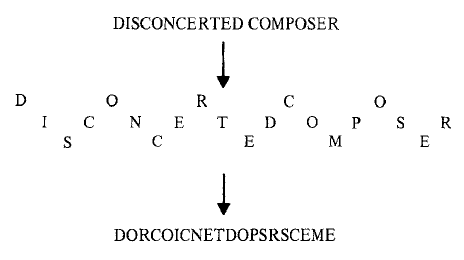
\includegraphics[width=0.65\textwidth]{./images/figExampleTranspositionCipher}
	\caption{Ejemplo de cifrado de transposición \citep{denning}.}
	\label{figExampleTranspositionCipher}
\end{figure}


Actualmente en los algoritmos que se implementan en computadoras se combina tanto la transposición como la sustitución. Por ejemplo se tiene el algoritmo RC5 (el cual se desarrollará más adelante en este proyecto), en donde se utiliza corrimientos o rotaciones a bits (transposición) y sumas o XOR's (sustituciones) para cifrar el texto plano. Los algoritmos que se implementan en la criptografía moderna se dividen en dos categorías principales: simétricos y de llave pública (también llamados asimétricos \citep{denning}).


\section{Algoritmos criptográficos}
\subsection{Algoritmos simétricos}
\cite{bruce} da una muy buena analogía para explicar el concepto de un algoritmo simétrico. Piense en el algoritmo como una caja fuerte. La combinación de la caja fuerte vendría a ser la \textit{llave} del algoritmo. Note como en una caja fuerte cualquier persona con la combinación puede llegar, abrir la caja y poner o sacar documentos de la misma. En el caso de no conocer la combinación, se debe proceder a forzar la caja o probando todas las combinaciones posibles hasta hallar la correcta. Es decir en un algoritmo simétrico se cuenta con una llave única que funciona tanto para cifrar como para descrifrar los mensajes como se muestra en la Figura \ref{figSimmetricKeyAlgorithm}. La notación para el cifrado y descrifado en estos algoritmos se muestra en las Ecuaciones \eqref{eqCifradoSimetrico} y \eqref{eqDescifradoSimetrico}.
\begin{equation}\label{eqCifradoSimetrico}
E_K (M) = C
\end{equation}

\begin{equation}\label{eqDescifradoSimetrico}
D_K (C) = M
\end{equation}


\begin{figure}
	\centering
	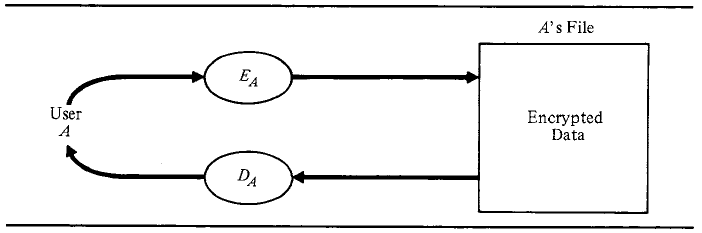
\includegraphics[width=0.9\textwidth]{./images/figSimmetricKeyAlgorithm}
	\caption{Descripción gráfica de una algoritmo de llave simétrica \citep{denning}.}
	\label{figSimmetricKeyAlgorithm}
\end{figure}


Los algoritmos simétricos se dividen en 2 categorías \citep{bruce}:

\begin{itemize}
\item Cifrado de bloque: Se cifra en bloques de bits ya sea \textit{bytes, words}, etc. Es decir cuando se va a proceder a cifrar un texto plano, se segmenta el texto en grupos de bits y estos son cifrados en conjunto. Se puede tomar como ejemplo el algoritmo \textit{Data Encryption Standart} (DES) el cual cifra sobre bloques de 64 bits. Otros ejemplos son:
\begin{itemize}
\item Lucifer.
\item LOKI.
\item 3-way.
\item RC5.
\item GOST.
\item IDEA.
\end{itemize}

\item Cifrado de \textit{Stream}: Es cuando se trabaja sobre un bit únicamente. Estos no son muy usuales en la actualidad ya que al trabajar en lenguaje binario solo se cuenta con 2 símbolos y si se cifra únicamente un bit no existen muchas posibilidades para sustituir o transposicionar.
Ejemplos de estos algoritmos pueden ser:
\begin{itemize}
\item RC4.
\item SEAL.
\item WAKE.
\end{itemize}
\end{itemize}

Según \cite{bruce}, los criptosistemas simétricos en la red afrontan los siguientes problemas
\begin{itemize}
\item Distribución de la llave: La llave se debe mantener en secreto. Esto en la actualidad es una tarea demasiado díficil de lograr porque la llave debe ser conocida para el cifrado y descifrado (emisores y receptores) entonces para establecer una comunicación segura el primer paso debe ser entregar la llave de forma segura, lo cual en una red de computadoras se puede tornar una tarea prácticamente imposible de realizar. La única solución sería entregar las llaves mediantes un servicio de \textit{courier} o similares e igualmente se corren riesgos. 

\item Compromiso de seguridad: Si la llave es conocida por un tercero, si este intercepta el tráfico de información, todas las comunicaciones serán descifradas fácilmente.

\item Comunicaciones aisladas: En el caso de que cada usuario de una red se desee comunicar secretamente por separado con todos los otros usuarios haciendo uso del mismo criptosistema, se debe utilizar una llave diferente para cada comunicación. Así para una red de N usuarios se requieren $N(N - 1)/2$ llaves. A primera vista esto no parece tan importante por ejemplo para 10 usuarios, se necesitan 45 llaves lo cual está bien, pero para 100 usuarios se necesitarían 4950 llaves que se tienen que distribuir de forma secreta.
\end{itemize}



\subsection{Algoritmos de llave pública}
Nuevamente \cite{bruce}, nos ofrece una excelente analogía para explicar, en este caso, los algoritmos de llave pública. Tenemos un \textit{mailbox}, donde cualquier persona puede poner un mensaje adentro pero \textbf{únicamente} el dueño puede abrirlo para sacar y leer los mensajes.
\newline
\newline
En los algoritmos de llave pública los emisores hacen uso de una llave para cifrar los mensajes que desean enviar pero estos mensajes pueden ser descrifrados únicamente si se tiene la llave para descifrar mensajes (que es diferente de la llave para cifrar), la cual el receptor la tendrá bien resguardada. En la Figura \ref{figPublicKeyAlgorithm} se muestra el diagrama básico de un algoritmo de llave pública. Ejemplos de estos algoritmos pueden ser:
\begin{itemize}
\item RSA
\item Pohlig-Hellman
\item Rabin
\item ElGamal
\end{itemize}

\begin{figure}
	\centering
	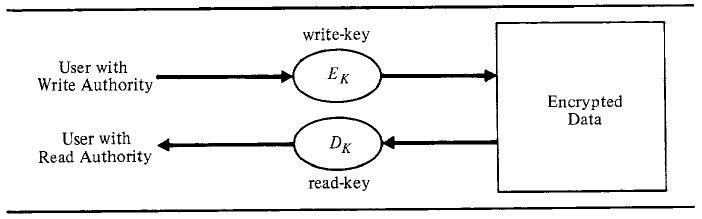
\includegraphics[width=0.65\textwidth]{./images/figPublicKeyAlgorithm}
	\caption{Descripción gráfica de una algoritmo de llave pública \citep{denning}.}
	\label{figPublicKeyAlgorithm}
\end{figure}

Estos algoritmos sientan su base matemática en funciones llamadas \textit{one-way} en donde al aplicarle una función a una variable, la variable no puede retornar a su valor original de ninguna manera, es decir la función no tiene una inversa. 

Según \cite{bruce}, existen funciones \textit{one-way} con una ``puerta trasera'' donde se puede retornar a la variable original conociendo ciertos parámetros, este tipo de funciones son las que se implementan en algoritmos de llave pública. Los algoritmos dominantes de esta rama se basan en la dificultad de factorizar números grandes que son el resultado de multiplicar dos números primos grandes como también se basan en el \textit{Discrete Logarithm Problem}.

En estos algoritmos no es posible a partir de la llave para cifrar obtener la llave para descrifrar. Esto permite que la llave para cifrar se pueda hacer pública, por lo cual recibe el nombre de llave pública y la llave para descrifrar se denomina llave privada. La notación para estos algoritmos corresponde a la de las Ecuaciones \eqref{eqCifradoPublico} y \eqref{eqDescfiradoPublico}
\begin{equation} \label{eqCifradoPublico}
E_{K_x} (M) = C
\end{equation}
\begin{equation} \label{eqDescfiradoPublico}
D_{K_y} (C) = M
\end{equation}

El objetivo de utilizar cifrado de llave pública se basa en:
\begin{itemize}
\item Receptor y emisor acuerdan un sistema criptográfico.
\item El receptor entrega al emisor su llave pública.
\item El emisor cifra el texto plano haciendo uso de la llave pública entregada y el sistema acordado.
\item El emisor envía el texto cifrado.
\item El receptor descrifa el texto cifrado haciendo uso de la llave privada.
\end{itemize}

De esta manera no hay forma en que fisgones logren descrifrar el mensaje aunque obtengan la llave pública. Así el receptor se asegura que las comunicaciones van a ser mucho más seguras, ya que el emisor deja de tener la llave para descifrar y no puede brindarsela a nadie o que le sea robada a este. Para la implementación de un criptosistema que hace uso de algoritmos de llave pública, lo que se hace es que en la red se tiene una base de datos donde se registra el usuario y su respectiva llave pública. Así cuando un usuario desea comunicarse con otro, va a la base de datos, busca al usuario y su llave pública, cifra el mensaje con la misma y se la envía. Esto solventa los problemas que presentaba anteriormente los algoritmos simétricos, ya que no es necesario transmitir de forma secreta llaves para poder realizar comunicaciones y para que diferentes usuarios se comuniquen de forma secreta entre si no es necesario el uso de diferentes llaves por cada enlace de comunicación. 

Algunos usos de estos algoritmos en la actualidad son:
\begin{itemize}
\item Llave maestra para el sistema de pago digital de un banco.
\item La clave que utiliza un gobierno para certificar sus visas o pasaportes.
\item La firma digital de un notario público.
\end{itemize} 

\subsection{Criptosistemas híbridos}
Los beneficios que conlleva utilizar algoritmos de llave pública son grandes pero se pagan a un precio muy alto: tiempo de procesamiento. Según \cite{bruce}, el tiempo de procesamiento del RSA con respecto al del DES es de alrededor de 1000 mil veces más lento. 

En un mundo donde la velocidad es una clave fundamental en las comunicaciones se propuso la siguiente solución. Ya que los algoritmos simétricos tienen la debilidad de comunicar la llave antes de comenzar la comunicación pero son mucho más rápidos, y que los algoritmos de llave pública ostentan una mejor sistema para comunicarse en la red secretamente pero son muy lentos, se decidió utilizar ambos. La llave del algoritmo simétrico es cifrado con un algoritmo de llave pública para transmistirse en la red sin comprometerla y posterior a esto se realizan las comunicaciones con el algoritmo simétrico para obtener una mejor velocidad de comunicación. Se puede ver el protocolo de la siguiente manera \citep{bruce}:
\begin{itemize}
\item El receptor envía su llave pública al emisor.
\item El emisor genera una llave de sesión\footnote{Una llave de sesión se utiliza en comunicaciones donde la idea es cifrar cada comunicación de manera individual con una llave distinta. Son útiles cuando la llave se crea al inicio de la comunicación y se destruye al final de la misma \citep{bruce}.}, la cifra y se la envía al receptor usando la llave pública que le fue dada.
\item El receptor descrifra la llave de sesión usando su llave privada.
\item Ahora ambos pueden comunicarse de forma secreta con la llave de sesión con un criptosistema simétrico.
\end{itemize}





\section{Seguridad en algoritmos criptográficos}
Como parte de la investigación previa para este proyecto no podemos dejar de lado la otra cara de la moneda, el criptoanálisis. La ciencia que abarca la criptografía y el criptoanálisis es conocida como criptología \citep{denning}. Claramente el objetivo de la criptografía es mantener un mensaje en secreto de terceros, pues el criptoanálisis según \cite{raeCriptoanalisis}, es el ``arte de descifrar criptogramas'', así es como los terceros buscan inmiscuirse en las comunicaciones secretas sin tener un acceso a la llave.  

Según \cite{bruce}, el criptógrafo al diseñar su algoritmo debe asumir que el criptoanalista puede tener un acceso completo a las comunicaciones entre emisor y receptor y al algoritmo que implementa el criptosistema, así toda la seguridad del criptosistema debe residir en la llave.

La acción en la que un criptoanalista atenta contra un criptosistema es denominada \textit{ataque}. Según \cite{bruce,denning}, los principales tipos de ataques son:
\begin{itemize}

\item \textit{Ciphertext-only}: El criptoanalista debe obtener la llave a partir de varios textos cifrados. Debe conocer el tema tratado de las comunicaciones que está interviniendo (lo cual es obvio, ya que sino para qué está interviniendo las comunicaciones) entonces puede saber de forma previa que ciertas cosas que puede contener el texto plano.

\item \textit{Known-plaintext}: El criptoanalista tiene acceso a ciertos textos planos y sus respectivos textos cifrados. A partir de estos debe deducir la llave o debe generar un algoritmo de descifrado equivalente al diseñado por el criptográfo.

\item \textit{Chosen-plaintext}: El criptoanalista puede obtener el texto cifrado de un texto plano que él seleccione, esto es mucho más poderoso porque puede cifrar mensajes que den más información acerca de la llave. Un sistema de bases de datos es vulnerable a este tipo de ataques debido a que los usuarios pueden agregar elementos a la base de datos y ver el resultado del texto cifrado en la misma. Nuevamente su tarea es obtener la llave o generar un algoritmo de descifrado equivalente.

\item \textit{Chosen-ciphertext}: Este tipo de ataque se da en algoritmos de llave pública, en donde el criptoanalista tiene acceso al texto cifrado que va a ser descifrado y al texto plano. Es decir tiene una ``caja negra'' donde la entrada es el texto cifrado y la salida el texto plano. El objetivo es obtener la llave a partir de estos recursos.

\item \textit{Chosen-key}: El criptoanalista tiene conocimiento sobre la relación entre las diferentes llaves.

\item \textit{Rubber-hose}: El criptoanalista amenaza, extorsiona, chantajea u obtiene de alguna forma la llave sin ningún tiempo.
\end{itemize}


Otro ejemplo es que los algoritmos de llave pública son vulnerables a ataques de tipo \textit{chosen-plaintext}. Tome por ejemplo M como un texto plano del espacio $M$ de posibles mensajes. La tarea de un criptoanalista es tomar todos $\text{M} \epsilon M$ y cifrarlos para obtener todos los posibles $\text{C} \epsilon C$. De esta manera solo debe interceptar las comunicaciones que desea y comparar sus valores de texto cifrado con los que intercepta para descifrar las comunicaciones. Note que el criptoanalista no pudo obtener la llave pero si logró descrifrar las comunicaciones.


\subsection{Tamaño de la llave} \label{secTamanoLlave}
Como se mencionó anteriormente la seguridad de un buen algoritmo depende de su llave. Asumiendo que se tiene una seguridad del algoritmo perfecta, la única forma de quebrar el criptosistema sería mediante un ataque de fuerza bruta, el cual es un tipo de ataque \textit{known-plaintext}, para obtener la llave. 

Analizando el tamaño de la llave, si se tuviera una de $2^8$ bits, probando las 256 posibilidades se obtendría la llave, lo cual equivale a unos cuantos segundos de procesamiento en una computadora. Para $2^{64}$ bits tenemos $1.8446744^{19}$ posibles llaves, lo cual tomaría con los recursos computacionales de una supercomputadora alrededor de 585,000 años. Para una llave de 2048, con un billón de intentos por segundo en computadoras en paralelo se necesitarían 10597 años para encontrar la llave \citep{bruce}. 


Entonces ¿Porqué no hacer un algoritmo con una llave muy grande?. La respuesta es porque conforme aumenta el tamaño de la llave, se paga en tiempo de procesamiento. Así se debe obtener un balance donde la llave sea lo suficientemente grande para que sea el algoritmo sea seguro, pero lo suficientemente pequeña para que el tiempo de procesamiento sea bueno \citep{bruce}.

Comparar el nivel de seguridad ante un ataque de fuerza bruta de un algoritmo simétrico y uno de llave pública con llaves del mismo tamaño no es posible, pero la Figura \ref{figVariacionLlaves} muestra una tabla con equivalentes realizados empíricamente por \cite{bruce} sobre tamaños de llaves que dan un nivel de seguridad equivalente para los dos tipos de algoritmos, esto nos indica que no es recomendable comparar algoritmos de distintas ramas entre sí.

\begin{figure}
	\centering
	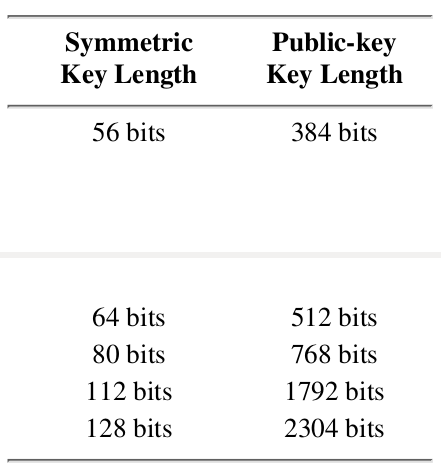
\includegraphics[width=0.65\textwidth]{./images/figVariacionLlaves}
	\caption{Comparación del tamaño de llaves en algoritmos simétricos y asimétricos \citep{bruce}.}
	\label{figVariacionLlaves}
\end{figure}

\subsection{Manejo de las llaves}
Se puede tener un algoritmo extremadamente robusto, veloz y con un tamaño de llave perfecto, pero si un atacante puede obtener la llave por algún medio el algoritmo es completamente inútil. De ahí la gran importancia de como manejar las llaves.

Al ser esto tan importante existen ciertas maneras de generar llaves:
\begin{itemize}
\item Ingresada por el usuario: El usuario elige una llave y esa es la que se va a utilizar. Este método es sumamente inseguro
debido a que gran cantidad de contraseñas se repiten, o son datos personales del usuario como su número de celular o similares.
Por tanto se pueden realizar \textit{ataques de diccionario} donde las primeras llaves que se prueban son las mencionadas
anteriormente.

\item \textit{Random keys}: Es un muy buen método para generar llaves, consiste en utilizar un programa que genere la llave, es ventajoso
ya que es robusto ante ataques de diccionario pero presenta el problema que la llave es difícil de recordar y posiblemente se olvide.

\item \textit{Pass phrases}: Es una combinación de ambos, el usuario escribe una contraseña fácil de recordar y después hace uso de una función \textit{one-way} el sistema convierte esta llave en una llave random de tamaño arbitrario.
\end{itemize}

\section{\textit{Field Programmable Gate Array} (FPGA)}
Un FPGA consiste en una matriz de bloques lógicos configurables, conectados mediantes interconexiones programables. Posterior al proceso de manufactura el FPGA puede ser reprogramado para darle una nueva funcionalidad, esto es lo que diferencia a un FPGA de un \textit{Application Specific Integrated Circuits} (ASIC) \citep{xilinx1}. 

\subsection{FPGA vs ASIC}
En años anteriores los FPGAs presentaban gran desventaja en cuanto a velocidad, consumo y área respecto a un ASIC y por eso aunque eran reprogramables, desarrollar aplicaciones en un FPGA solo se daba para realizar prototipos y no para un producto final. En la actualidad los FPGAs se encuentran en auge debido a que su proceso de manufactura ha mejorado mucho en los aspectos anteriormente descritos, por ejemplo un FPGA ya puede alcanzar los 500MHz, han aumentado la densidad de lógica y albergan otras funcionalidades como por ejemplo módulos de \textit{Digital Signal Proccessing} (DSP), de tiempos y hasta de \textit{high-speed serial} \citep{xilinx1}.

Estos grandes avances en conjunto con un flujo de diseño mucho más fácil, barato y rápido, indican que el desarrollo en FPGAs va a convertirse en la nueva forma de diseñar hardware. La Tabla \ref{tablaFPGA} muestra beneficios y ventajas del diseño con FPGAs y la Figura \ref{figFpgaVsAsic} muestra la diferencia en el ciclo de diseño de hardware con FPGAs y ASICs. Aún con todas estas ventajas los FPGAs todavía presentan ciertas desventajas con respecto a los ASICs, como se muestra en la Tabla \ref{tablaASIC}.


\begin{table}[]
\centering
\caption{Ventajas y beneficios de diseñar con FPGAs \citep{xilinx3}.}
\label{tablaFPGA}
\begin{tabular}{l|l}
Ventaja                                 & Beneficio                                                                                                          \\ \hline
Tiempo de producción más corto      & \begin{tabular}[c]{@{}l@{}}Pasos de manufactura como layout, \\ máscara u otros  no son necesarios\end{tabular}                \\
No upfront non-recurring expenses (NRE) & Costo que ocurre en el diseño de ASICs.                                                                     \\
Ciclo de diseño más simple                    & \begin{tabular}[c]{@{}l@{}} El software se encarga en gran parte del \\ \textit{placing, routing} y \textit{timing.}\end{tabular} \\
Ciclo del proyecto más predecible          & \begin{tabular}[c]{@{}l@{}}Debido a que se eliminan los posibles \\ re-spins, capacidades de la oblea, etc.\end{tabular}        \\
\textit{Field reprogramability}                  & Se puede cargar un nuevo RTL y listo.                                                                            
\end{tabular}
\end{table}


\begin{figure}
	\centering
	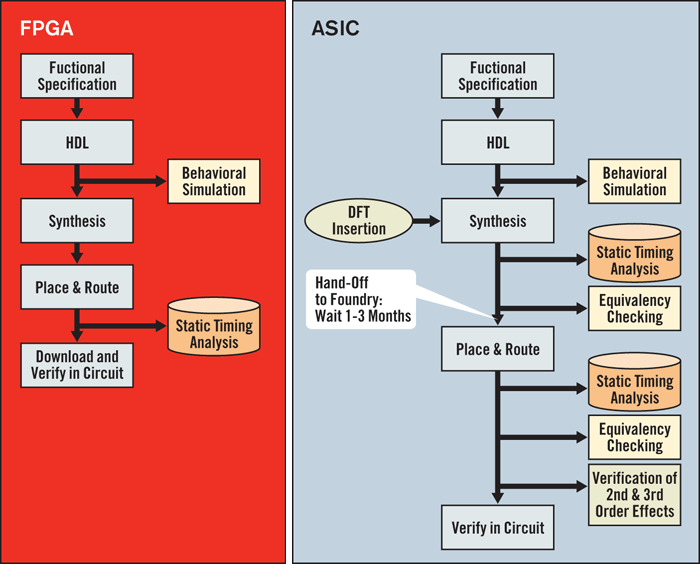
\includegraphics[width=0.9\textwidth]{./images/figFpgaVsAsic}
	\caption{Ciclo de diseño de hardware para FPGAs y ASICs \citep{xilinx3}.}
	\label{figFpgaVsAsic}
\end{figure}

\begin{table}[]
\centering
\caption{Ventajas y beneficios de diseñar con ASICs \citep{xilinx3}.}
\label{tablaASIC}
\begin{tabular}{l|l}
Ventaja                & Beneficio                                                                                          \\ \hline
100\% personalizados & \begin{tabular}[c]{@{}l@{}}Ya que se manufactura \\ apegado a la especificación.\end{tabular} \\
Costos unitarios más bajos       & Para diseños de gran volumen.\\
Más pequeños    & \begin{tabular}[c]{@{}l@{}}Debido a que el diseño se acoge \\ completamente a la especificación.\end{tabular}
\end{tabular}
\end{table}





\subsection{Componentes básicos de un FPGA}
Todos los FPGAs, como se muestra en la Figura \ref{figEstructuraFPGA}, tiene como mínimo 3 componentes \citep{xilinx2}
\begin{itemize}
\item \textit{Configurable Logic Block}
\item \textit{Programmable Switching Matrix}
\item \textit{Input/Output Block}
\end{itemize}

\begin{figure}
	\centering
	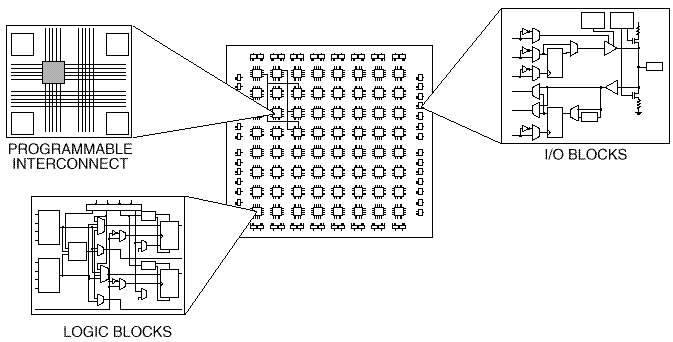
\includegraphics[width=0.9\textwidth]{./images/figEstructuraFPGA}
	\caption{Estructura básica de un FPGA. \citep{figRandom1}}
	\label{figEstructuraFPGA}
\end{figure}

A parte de estos componentes un FGPA también puede tener un módulos de memoria RAM, ROM y hasta módulos para DSP.

A continuación se describen de forma general los componentes que conforman los bloques descritos anteriormente \citep{xilinx2,xilinx4}
\begin{itemize}

\item \textit{Configurable Logic Block} (CLB): Corresponde a la unidad principal de diseño para lógica combinatoria y flip-flops. Se encuentra compuesto por slices y la cantidad que lo componen varía según el modelo. Para determinar la densidad de slices por CLB se debe sintetizar el diseño previamente para decidir cual es el modelo que se ajusta al mejor desempeño del diseño. Estos bloques son conectados a un PSM para comunicarse con otras partes del FPGA y también se conectan a un IOB para comunicarse con el mundo exterior. La Figura \ref{figEstructuraCLB} muestra una representación general de lo que puede contener un CLB.

\begin{figure}
	\centering
	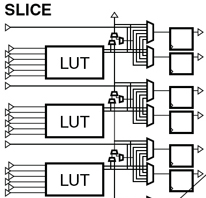
\includegraphics[width=0.4\textwidth]{./images/figEstructuraCLB}
	\caption{Estructura básica de un CLB \citep{xilinx5}.}
	\label{figEstructuraCLB}
\end{figure}

\item \textit{Slice}: Es la unidad básica de un FPGA, puede estar compuesto por:

\begin{itemize}
\item \textit{Look Up Table} (LUT): También son llamados Function Generators, depende del número de entradas y no de la complejidad de la función que se está implementando. Así el retardo es constante para todo el LUT. Son usados para implementar lógica booleano y también como memoria o SRL\footnote{Shift Register Lookup Table (SRL) es un registro desplazable de tamaño variable. Sus usos pueden ser como retardo programable o como una memoria FIFO.}

\item \textit{Wide Multiplexers}: Se utilizan para conectar LUTs entre si y también para no utilizar LUTs en operaciones simples, ahorrando LUTs y mejorando la velocidad de procesamiento. 
\item \textit{Carry Chain}: Cuando los CLBs deben de realizar operaciones como sumas o restas utilizan esta característica para mejorar la velocidad en la que se realiza la operación
\item \textit{Registers}: Pueden ser flip-flops o latches.
\end{itemize}

Ciertos slices pueden se utilizados como una memoria RAM distribuida, en donde por ejemplo el LUT se utiliza como una memoria, ya sea en configuración \textit{single, dual, simple-dual o quad port}. 

\item \textit{Programmable Switch Matrix} (PSM): Corresponde a un módulo en donde se realiza la interconexión de los distintos CLBs y otros componentes del FPGA según requiera el diseño. Esta interconexión puede realizarse de forma vertical, horizontal y diagonal.


\item Input/Output Blocks (IOB): Estos bloques se encargan de comunicar al FPGA con el mundo exterior, manejan gran cantidad de estándares de comunicación como por ejemplo: LVCMOS, PCI, I2C y SSTL.
\end{itemize}


Como se puede observar los FPGAs son de gran importancia y por eso el objetivo de implementar los algoritmos criptográficos en un FPGA adquiere relevancia. Así también es muy importante conocer que tantos recursos (slices, memoria y DSP) se requieren para implementar estos diseños en un FPGA ya que al aumentar la cantidad de recursos aumentan los costos de producción, volviendo este proyecto relevante por su proyección innovadora sin dejar de lado el aspecto económico tan importante en la industria. 






\section{Escogencia de los algoritmos a implementar}
En un principio el objetivo de este proyecto era realizar una comparación con las métricas descritas en la Introducción sobre un algoritmo simétrico y un algoritmo de llave pública, posterior a la realización del marco teórico se llegó a la conclusión de que realizar este análisis no iba a ser para nada justo debido a tres razones:

\begin{itemize}
\item El tiempo de procesamiento: Como se menciona anteriormente los algoritmos de llave pública consumen mucho más tiempo realizando el cifrado y descifrado que un algoritmo de llave simétrica.

\item La formas en las que estos algoritmos son diseñados producen falencias en seguridad distintas, como se indica en la sección \ref{secTamanoLlave} los tamaños de llaves varían mucho para lograr una seguridad similar ante un ataque de fuerza bruta, esto haría poco justo realizar un análisis comparativo con el mismo tamaño de llave.

\item Los algoritmos realizan el proceso de cifrado de maneras muy diferentes: En el caso de los algoritmos simétricos son basados en transposición y sustitución que trabajan en su mayoría con XOR's, sumas y corrimientos. En cambio los algoritmos de llave pública trabajan  basados en la multiplicación de números primos y \textit{Discrete Logarithm Problem} donde ocurren muchas multiplicaciones y sumas. Esto produce un consumo de recursos muy diferente entre ambos tipos.
\end{itemize}

Bajo el criterio que ambos algoritmos tuvieran características similares para poder ser analizados comparativamente y que fueran fáciles de implementar a nivel de hardware se optó por comparar dos algoritmos simétricos, específicamente el RC5 y el TEA los cuales están basados en redes de Feistel\footnote{
Las redes Feistel toman un bloque de texto plano de tamaño N (par) y lo dividen en dos mitades denominadas L y R. El cifrado en este tipo de redes es iterativo donde el resultado de la iteración $i$ depende del resultado de la iteración $i - 1 $. Ejemplos de algoritmos de este tipo pueden ser DES, Lucifer, FEAL, Khufu, Khafre, LOKI, GOST, CAST, Blowfish, entre otros.} y por tanto comparten características de diseño para que la comparación sea un poco más justa.





\section{Descripción de los algoritmos a implementar}
\subsection{RC5}
El algoritmo criptográfico de llave simétrica RC5 fue creado en 1997 por Ronald Rivest para la \textit{RSA Data Security}. Según \cite{rivest} los objetivos de este algoritmo se basaban en que fuera adaptable tanto para hardware como para software, que tuviera una llave de tamaño variable, que el tamaño de la palabra a cifrar fuera de tamaño variable para que así se ajustara a procesadores de tamaños de palabra diferentes y por último que el número de rondas de cifrado fuera variable (con la finalidad de permitir decidir que tanta seguridad y que tan rápido se cifran los datos).

\subsubsection{Terminología del algoritmo}
Por simplicidad como se tienen tantos parámetros variables para el algoritmo entonces a la hora de llamarlo se utiliza la siguiente notación: RC5-w/r/b. Estas y otras variables se definen a continuación:

\begin{itemize}
\item w: es el tamaño de la palabra, el valor nominal es de 32 bits y los permitidos son 16 bits, 32 bits y 64 bits. Y el algoritmo cifra en bloques de tamaño 2w. Además cada palabra contiene $u=w/8$ bytes.

\item r: corresponde al número de rondas, los cuales pueden variar entre 0 y 255. Esto debido a que el algoritmo se basa en una red Feistel.
 
\item S: tabla con la expansión de la llave. Tiene un tamaño de $t= 2(r+1)$ palabras.

\item llave: Se tiene dos parámetros para definirla:
\begin{itemize}
\item b: cantidad de bytes que tiene la llave.
\item K[i]: K-ésimo byte de la llave va desde K[0] hasta K[b-1].
\end{itemize}

\item A y B: Corresponden a las partes izquierda y derecha del texto plano respectivamente.

\item L: Arreglo de $c=max(b,1)/u$ palabras que funciona para convertir la llave de bytes a palabras. Inicialmente se encuentra lleno de ceros.

\item $P_w$ y $Q_w$: Constantes que se definen como:
\begin{equation}
P_w = odd(2^w(e-2)); \text{   }e = \text{número de euler}
\end{equation}
\begin{equation}
Q_w = odd(2^w(\phi-2));\text{   } \phi = \text{golden ratio}
\end{equation}
\end{itemize}



Según \cite{rivest} los beneficios de utilizar el RC5 como algoritmo de cifrado se tiene una serie de parámetros variables los cuales conforme pasa el tiempo se pueden adaptar a la necesidades de cifrado. Un ejemplo de lo necesario que es esto es el problema con el algoritmo DES , para cuando fue creado su tamaño de llave era ideal pero ahora es muy corta y no hay forma fácil de que el algoritmo acepte una más fácil.

Otros usos del algoritmo es por ejemplo \citep{rivest} RC5-32/8/0, es decir si el uso de una llave, para generar una secuencia de números pseudo-aleatorios.


También es importante destacar que:
\begin{itemize}
\item + indica suma complemento a dos. Así como - indica resta en complemento a dos.
\item $\oplus$ indica un XOR bit a bit.
\item $<<<$ indica rotación hacia la izquierda, igualmente $>>>$ indica rotación a la derecha. Entonces X $<<<$ Y significa que la palabra X se rota Y bits a la izquierda.
\end{itemize}

\subsubsection{Pasos del algoritmo}
A continuación se muestra el pseudo-código extraído de \cite{rivest} para cifrar y descifrar datos con este algoritmo. 
\begin{itemize}
\item Expansión de llave: Corresponde la primer paso antes de poder cifrar o descifrar texto plano. Recibe como entrada una llave de tamaño arbitrario y realiza lo siguiente:
\begin{lstlisting}[mathescape]
for i = b - 1 downto 0 do
	L [i/u] = (L[i/u] <<< 8) + K[i]
	
S[0] = Pw;

for i = 1 to t-1 do
	S[i] = S[i-1] + Qw;
	
i = j =0
A = B =0

do 3*max(t,c) times:
	A = S[i] = (S[i] + A + B) <<< 3
	B = L[j] = (L[j] + A + B) <<< ( A + B )
	i = (i+1) mod(t)
	j = (j+1) mod(c)
\end{lstlisting}
Esto lo realiza para transformar la llave de bytes a palabras que se guardan en el arreglo S para que cada palabra de este arreglo se utilice para cifrar o descifrar el texto plano.

\item Cifrado: se realiza sobre los bloques de texto plano A y B simultáneamente, se realizan operaciones XOR y rotaciones entre el texto plano y palabras del arreglo S:
\begin{lstlisting}[mathescape]
A = A + S[0];
B = B + S[1];

for i = 1 to r do
	A = ((A $\oplus$ B) <<< B) + S[2i];
	B = ((B $\oplus$ A) <<< A) + S[2i + 1];
\end{lstlisting}


\item Descifrado: se realiza sobre los bloques cifrados A y B simultáneamente y se aplica las operaciones inversas a las del cifrado:
\begin{lstlisting}[mathescape]
for i = r downto 1 do
	B = ((B - S[2i + 1]) >>> A) $\oplus$ A;
	A = ((A - S[2i]) >>> B) $\oplus$ B;
	
B = B - S[1];
A = A - S[0];
\end{lstlisting}
\end{itemize}




\subsection{TEA}




\chapter{Implementación de los algoritmos}

\section{Implementación algoritmo RC5}
La implementación se basó en el siguiente análisis:
\begin{itemize}
\item Se tienen parámetros variables y el objetivo del proyecto es poder analizar como la variación de los mismos impacta en la utilización de recursos del FPGA. Por tanto la manera más óptima de generar código en Verilog es que el código sea parametrizable.

\item Se tiene arreglos de palabras los cuales son de tamaño variable de donde se leen y se escriben valores. La mejor forma de implementar esto es haciendo uso de memorias.

\item Usualmente para cada paso del algoritmo se debe realizar lo siguiente:
\begin{itemize}
\item Se lee un dato.
\item Se opera sobre el dato.
\item Se guarda el dato.
\item Se verifica si ya se terminaron de operar todo los datos.
\item Se cambia o mantiene la dirección para leer otro dato.
\end{itemize}
Tomando esto en consideración se optó por implementar máquinas de estado finitas para poder segmentar fácilmente los pasos a seguir y que los mismos sean manejados mediante un reloj.

\item Se tienen rotaciones hacia la izquierda y la derecha de N sobre M bits. Donde N es un valor calculado en tiempo de ejecución sobre una palabra de tamaño M. Esto se podría lograr mediante un barrel shifter que se genere dependiendo de los parámetros enviados a la hora de sintetizar, pero se consideró muy complicado y poco necesario. Por tanto se fijaron 3 tamaños de palabra comunes sobre los cuales se van a realizar los análisis: 16 bits, 32 bits y 64 bits. Esto facilita la escritura de código realizando un barrel shifter específico para cada tamaño de palabra. 

\item Se tienen sumas y restas de complemento a dos las cuales se ajustan perfectamente al uso de sumadores del FPGA.

\item Se tiene XOR bit a bit que se ajustan perfectamente a una implementación en hardware.
\end{itemize}

A partir de esto podemos concluir que:
\begin{itemize}
\item Los arreglos L, S y el arreglo de K[0] a K[b-1] corresponden a memorias RAM.
\item Cada uno de los \textit{for} que muestran en el pseudo-código corresponde a una máquina de estados la cual está controlada por un contador para manejar la cantidad de iteraciones.
\end{itemize}
Finalmente a partir de todos estos razonamientos se obtuvieron los diagramas de bloques para el cifrado y descifrado que se muestran en las Figuras \ref{figCipherBlockDiagram} y \ref{figDecipherBlockDiagram} respectivamente.

\begin{figure}
	\centering
	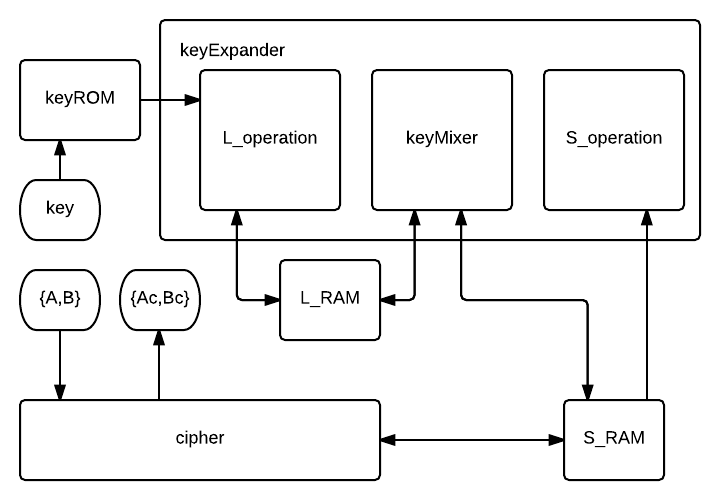
\includegraphics[width=0.7\textwidth]{./images/figCipherBlockDiagram}
	\caption{Diagrama de bloques del algoritmo de cifrado RC5.}
	\label{figCipherBlockDiagram}
\end{figure}
\begin{figure}
	\centering
	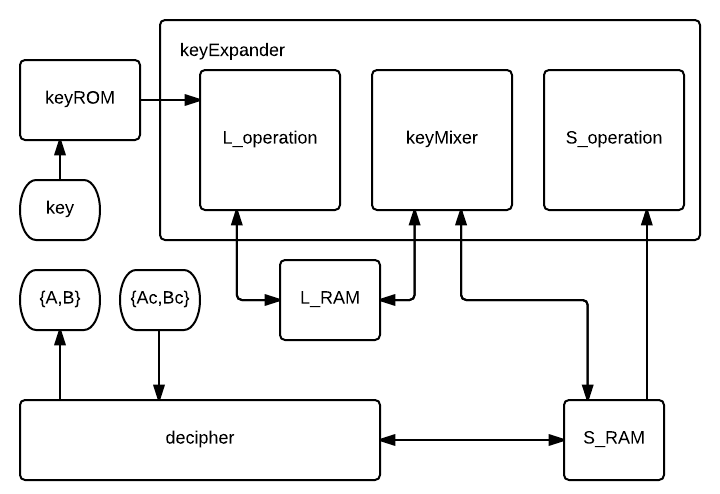
\includegraphics[width=0.7\textwidth]{./images/figDecipherBlockDiagram}
	\caption{Diagrama de bloques del algoritmo de descifrado RC5.}
	\label{figDecipherBlockDiagram}
\end{figure}


Cada bloque representa un ROM o RAM donde esté indicado y los demás corresponden a máquinas de estados finitas. El diagrama de estados para los bloques \textit{L\_operation, S\_operation} se muestra en la Figura \ref{figSL_operationFSM}. Note que ambos bloques comparten el diagrama de estados pero realizan diferentes operaciones. Para los bloques \textit{keyMixer, cipher y decipher} los diagramas de estados se muestran en las Figuras \ref{figKeyMixerFSM}, \ref{figCipherFSM} y \ref{figDecipherBlockDiagram} respectivamente.

\begin{figure}
	\centering
	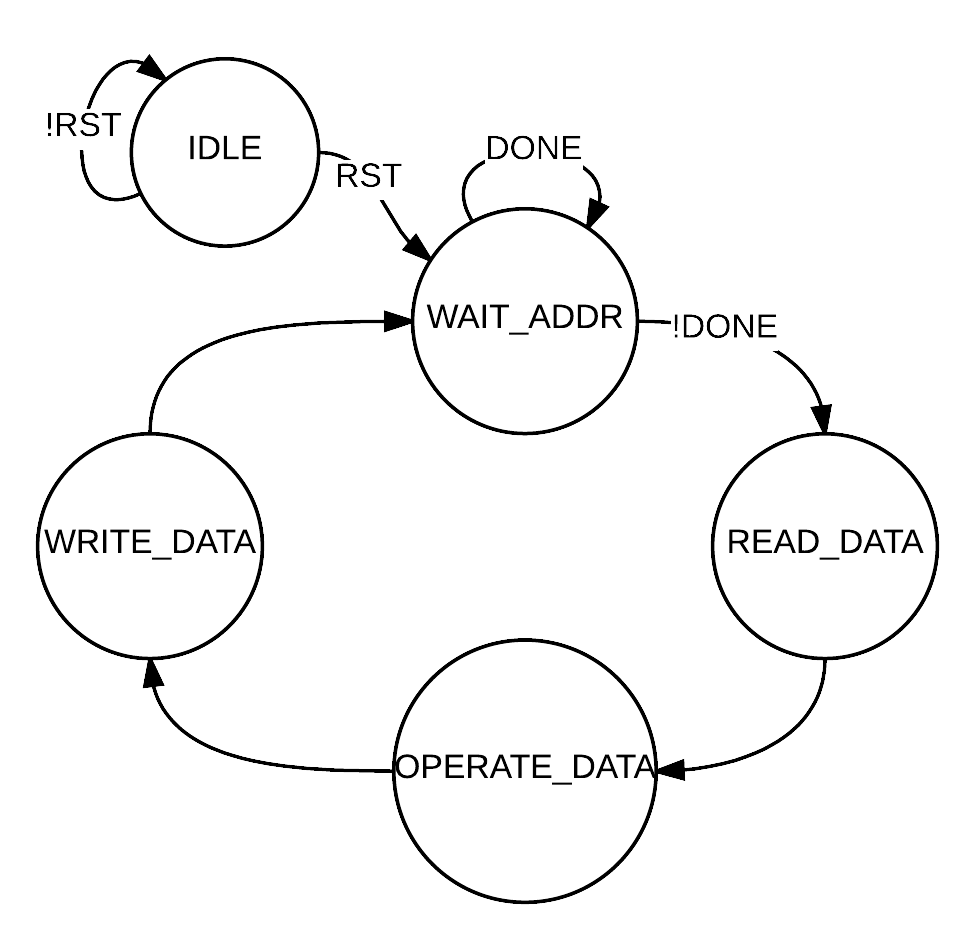
\includegraphics[width=0.5\textwidth]{./images/figSL_operationFSM}
	\caption{Diagrama de estados para los bloques \textit{L\_operation} y \textit{S\_operation}.}
	\label{figSL_operationFSM}
\end{figure}
\begin{figure}
	\centering
	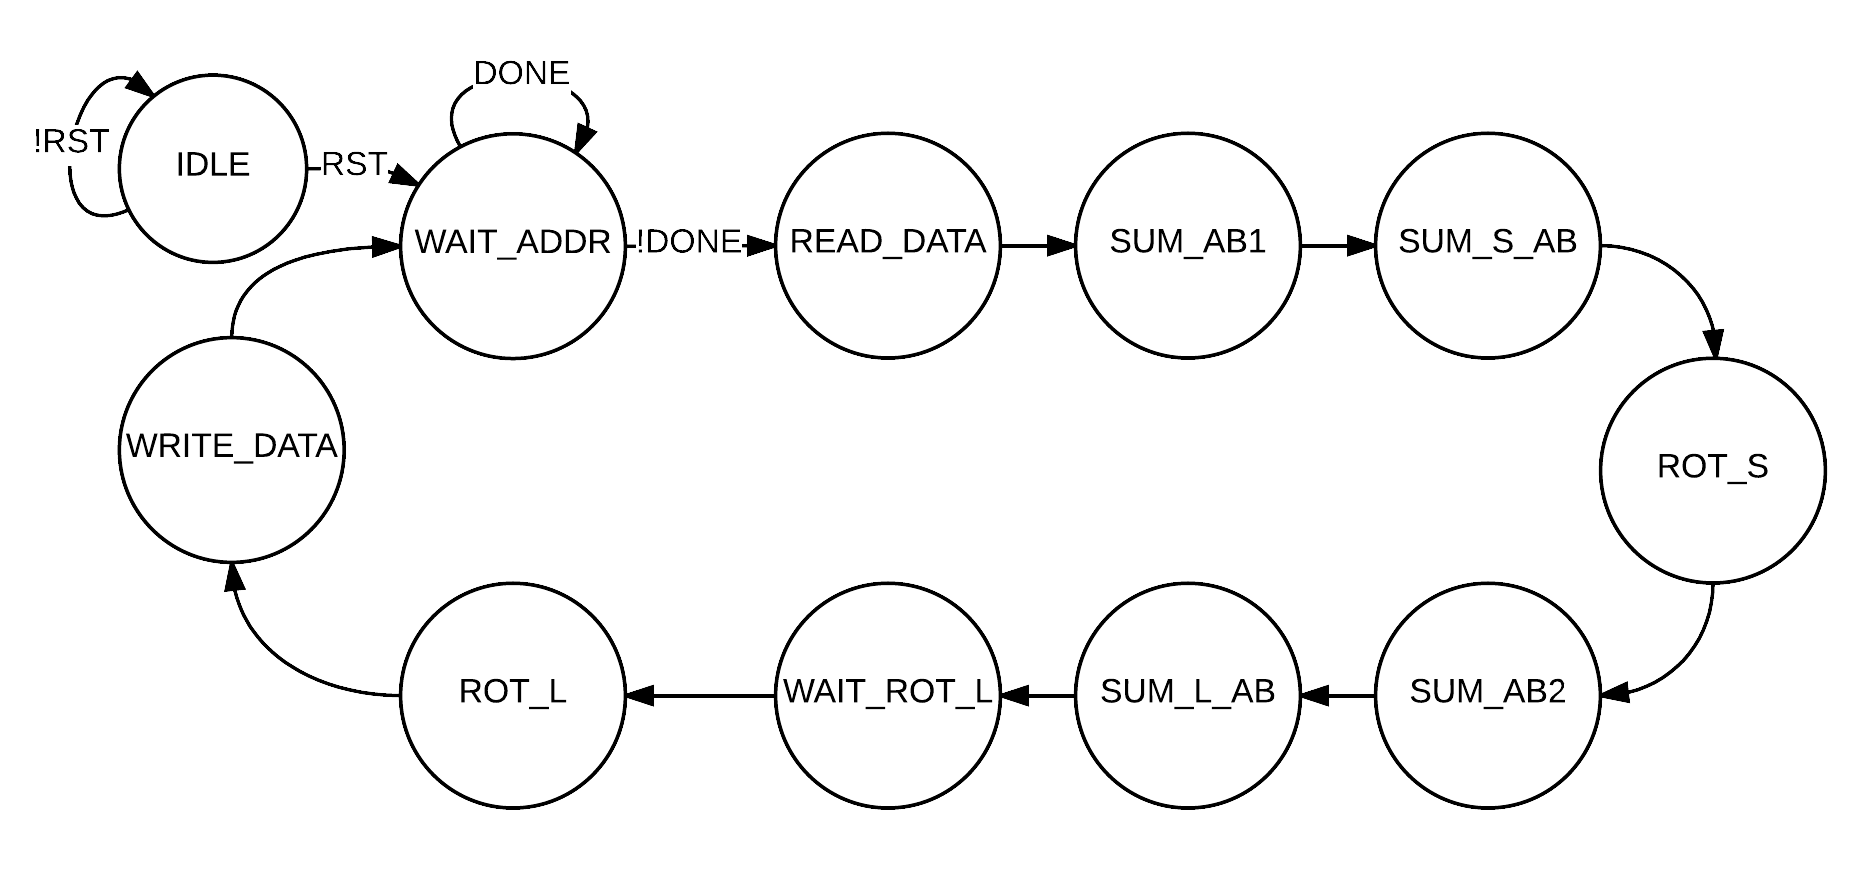
\includegraphics[width=0.85\textwidth]{./images/figKeyMixerFSM}
	\caption{Diagrama de estados para el bloque \textit{keyMixer}.}
	\label{figKeyMixerFSM}
\end{figure}
\begin{figure}
	\centering
	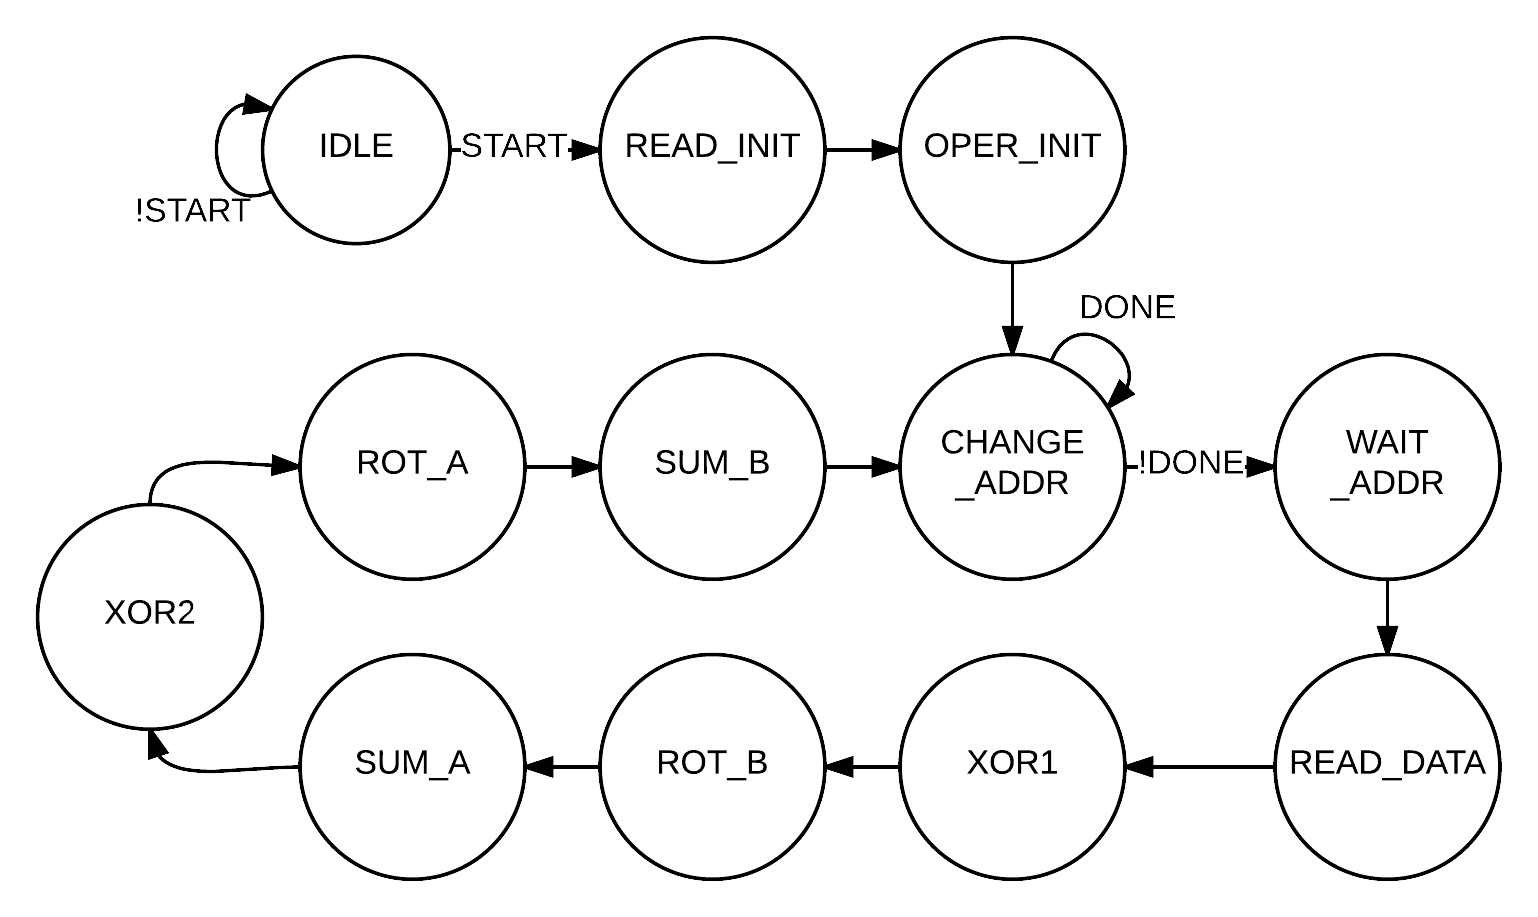
\includegraphics[width=0.85\textwidth]{./images/figCipherFSM}
	\caption{Diagrama de estados para el bloque \textit{cipher}.}
	\label{figCipherFSM}
\end{figure}
\begin{figure}
	\centering
	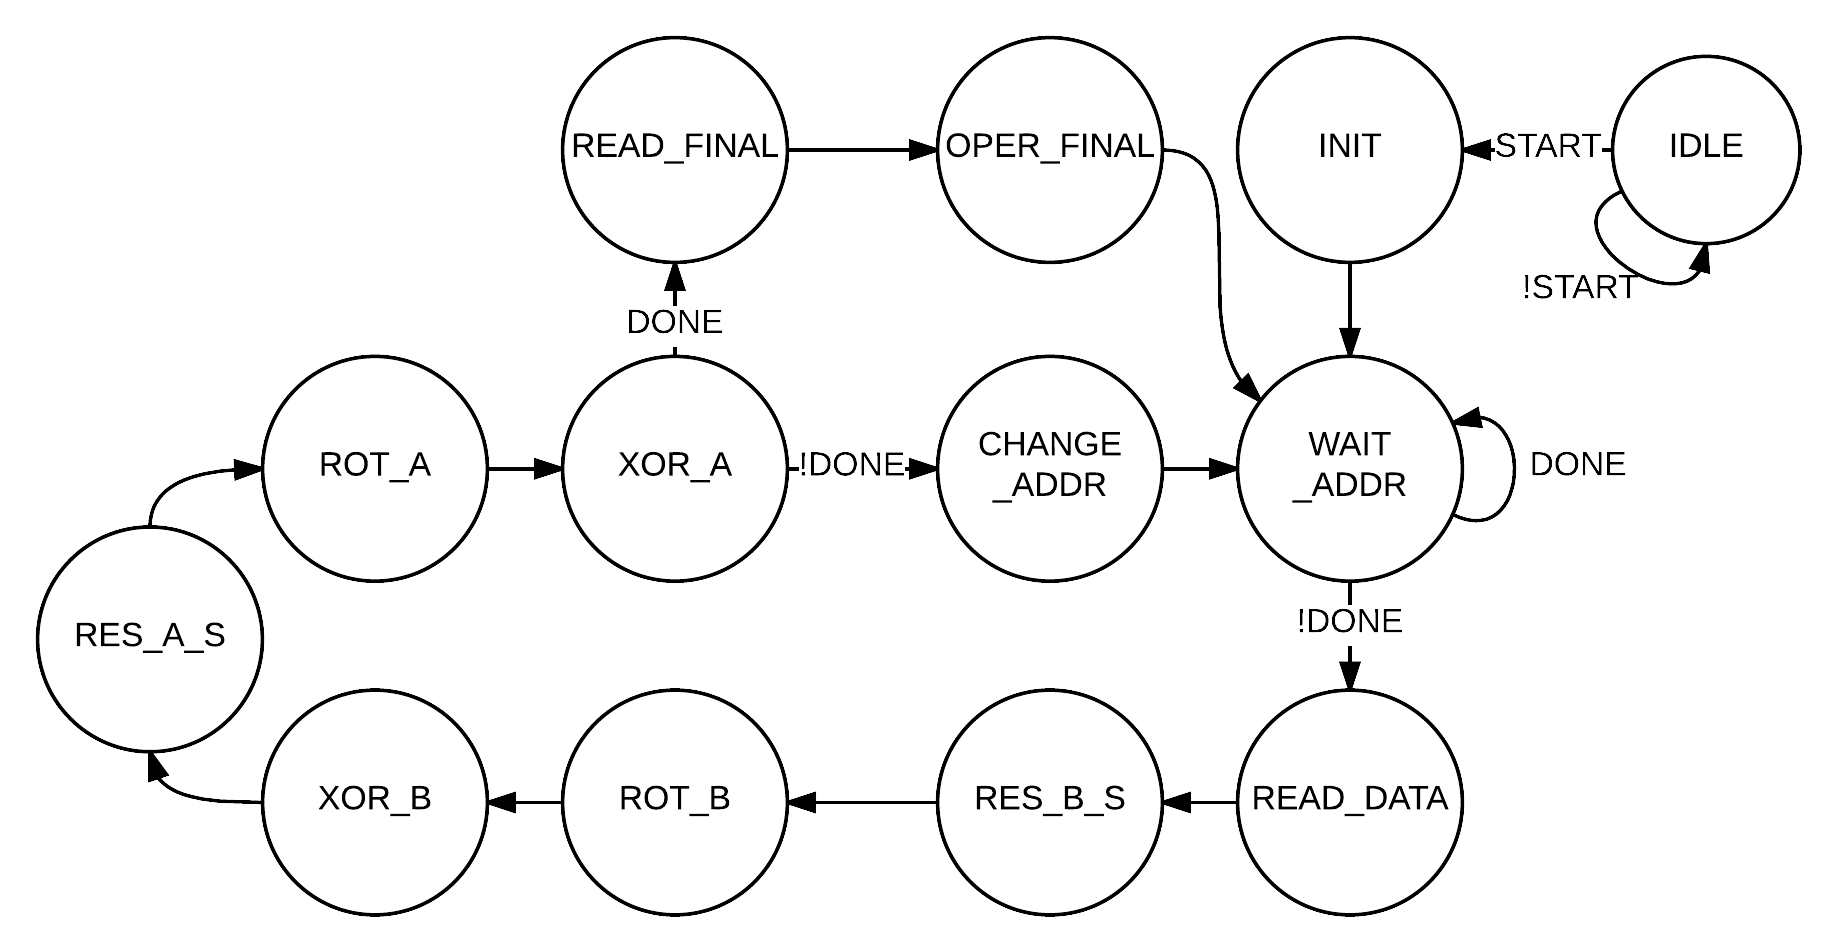
\includegraphics[width=0.85\textwidth]{./images/figDecipherFSM}
	\caption{Diagrama de estados para el bloque \textit{decipher}.}
	\label{figDecipherFSM}
\end{figure}

Un punto importante a aclarar es que el \textit{keyROM} de las Figuras \ref{figCipherBlockDiagram} y \ref{figDecipherBlockDiagram} se sintetiza en los resultados ya que por facilidad se optó por dejar el mismo como una entrada al circuito diseñado.


\section{Implementación del algoritmo TEA}
\blindtext
\cleardoublepage







\chapter{Resultados y análisis}

\section{Resultados y análisis del algoritmo RC5}
\blindtext
\cleardoublepage

\section{Resultados y análisis del algoritmo TEA}
\blindtext
\cleardoublepage

